\newpage
\section{Аналитический раздел}
В данном разделе рассмотрены: процесс обработки прерываний;
процедуры доступа к портам ввода/вывода;
драйвер символьного устройстваю;
подсистема ввода ядра.

\subsection{Процесс обработки прерываний}
Прерывание - это сообщение, информирующее систему о том, что одно из устройств выполнило операцию или на нем произошла ошибка. 
Прерывание заставляет процессор приостановить выполнение программы и вызвать операционную систему, чтобы иметь возможность ответить на прерывание \cite{3}.
Прерывания могут быть сгруперованы в две категории в зависимости от источника прерывания:
\begin{enumerate}
	\item синхронные прерывания или внутренние (исключения) - генерируются при выполнении иснтрукции.
	Они обрабатывают условия, обнаруженные процессором при выполнении инструкции;
	\item асинхронные прерывания - являются классическим типом прерываний и вызываются периферийными устройствами в произвольное время. 
	В отличие от синхронных прерываний, асинхронные не связаны каким-нибудь процессом. 
	Они возникают в любое время независимо от состояния системы и легко выполнимы.
\end{enumerate}

\subsubsection{Контроллер прерываний}
Устройство, поддерживающее прерывания, имеет выходной контакт используемый для отправки запроса прерывания (IRQ). 
Каждый из этих контактов называется линией прерывания и подключен к устройству под названием Контролер прерывайний (Programmable Interrupt Controllet, PIC), которое подключено к контакту intr процессора. Схема контролера прерываний показана на рисунке \ref{fig:interupt-device}.

\begin{figure}[H]
	\centering
	\includegraphics[width=0.7\linewidth]{"src/img/interupt device"}
	\caption{Схема контролера прерываний}
	\label{fig:interupt-device}
\end{figure}

\subsubsection{Обработчик прерываний}
Как и с другими ресурсами, преред тем как и их использовать, модуль запрашивает канал прерывания (IRQ) и так же особождает его, когда заканчивает работу.
Во многих случиях ожидается, что модули будут способны делить линии прерывания с другими драйверами.

В Linux запрос на получение и особождение прерывания выполняется с помощью функций request\_irq() и free\_irq объявленных в <linux/interrupt.h> (листинг \ref{lst:irq})
\begin{lstlisting}[caption={Функция request\_irq() и free\_irq()}, label={lst:irq}]
int request_irq(unnsigned int irq_no,
				irqreturn_t (*handler)(int, void *, struct pt_regs *),
				unsigned long flags,
				const char *dev_name,
				void *dev_id);

void free_irq(unsigned int irq_no, void *dev_id);
\end{lstlisting}

После того как прерывание было запрошено, оно будет обработано функцией обработчика.

\subsection{Отложенное действие}
Отложенное действие - это класс средст ядра, который позволяет планировать выполнение кода на более позднее время.
Оно используется для дополнения функциональности обработчика прерываний.
При использовании отложенного действия минимальная требуемая работа выполняется в обработчике прерываний, а остальные операции будут запланированы из обработчика прерываний для выполнения позже. 

В настоящее время существует 3 механизма отложенного действия:
\begin{enumerate}
	\item softirqs - могут использоваться драйверами устройств и зарезервированы для подсистем ядра;
	\item тасклеты - они работают в контексте прерывания, как и softirqs.
	Основное отличие заключается в том, что тасклеты могут выделяться динамически и, следовательно, использоваться драйверами устройств.
	\item очереди работ - используются для планирования действия, выполняемых в контексте процесса.
\end{enumerate}

В работе планируется использовать IRQ1 (контролер клавиатуры) для захвата прерываний с клавиатуры

В данной работе будет будем использовать тасклет, поскольку он работает относительно быстрее очереди работ. 
Так же он может быть использован в драйвере устройства в отличии от softirq

\subsection{Процедуры доступа к портам ввода/вывода}
В Linux доступ к портам ввода-вывода реализован на всех архитектурах, и существует несколько API, которые можно использовать.

Перед доступом к портам ввода-вывода необходимо вызвать запрос доступа, чтобы убедиться, что существует только один пользователь. 
Для этого используется функция request\_region(). 
Чтобы освободить зарезервированную область, необходимо использовать функцию release\_region().

После получения нужного порта ввода-вывода на нем можно выполнять операции чтения или записи. 
Поскольку физические порты различаются по количеству битов (8, 16 или 32 бита), существуют различные функции доступа к портам в зависимости от их размера. 
В asm/io.h определены следующие функции доступа к портам:
\begin{enumerate}
	\item unsigned inb(int port): чтение одного байта из порта;
	\item void outb(unsigned char byte, int port): запись одного байта в порт;
	\item unsigned inw(int port): чтение двух байтов из порта; 
	\item void outw(unsigned short word, int port): запись двух байтов в порт; 
	\item unsigned inl(int port): чтение четырех байтов из порта; 
	\item void outl(unsigned long word, int port): запись четырех байтов в порт. 
\end{enumerate}

\subsection{Драйвер символьных устройств}
В UNIX доступ к аппаратным устройствам осуществляется пользователем через специальные файлы устройств. 
Эти файлы группируются в каталог /dev, а системные вызовы open, read, write, close, и т. д. перенаправляются операционной системой на драйвер устройства, связанный с физическим устройством.
Драйвер устройства – это компонент ядра (обычно модуль), которая предназначена для управления конкретным устройством. 
Обычно драйверы устройств содержат последовательность команд, специфичных для конкретного устройства. 
Поскольку драйвер предназначен управления устройством, то код должен соответствовать специфике устройства. 
Обычно это связано с форматом передачи данных от системы к устройству и обратно.

В системах UNIX все устройства разделены на два типа \cite{5}:
\begin{enumerate}
	\item блочные - блочное устройство хранит данные и производит ввод-вывод блоками фиксированного размера, доступными в произвольном порядке.
	Обычно размер блока равняется 512 байтам, умноженным на 2 в степени, где степень больше либо равно 0.
	В качестве примеров блочных устройств можно указать жесткие диски, привод компакт-дисков \cite{5};
	\item символьные - символьные устройства могут использоватсья для хранения и передачи данных произвольного объема. 
	Некоторые устройства этого типа умеют передавать информацию побайтно, вырабатывая каждый раз прерывание.
	Данные устройства не в состоянии использовать произвольную адрисацию и не поддерживают операцию поиска.
	Примерами устройств такого типа являются терминалы, принтеры, "мыши" и звуковые карты \cite{5}.
\end{enumerate}

\subsubsection{Старший и младший номера устройств}
Индетификация и обращение к устройствам определяется пространством имен устройств.
В системе Unix существует три различных пространста имен устройств:
\begin{enumerate}
	\item аппаратное пространство;
	\item ядро;
	\item пользовательское.
\end{enumerate}

Ядро индетифицирует устройство по типу (блочное или символьное), а также по паре номеров, получивших название старжего и младшего номера устройств (major или minor).
Старший номер устройства идинтифицирует его драйвер. 
Младший номер устройства идентифицирует определенный экземпляр устройства \cite{5}.

\subsubsection{Структуры данных символьного устройства}
В ядре устройство символьного типа представлено структурой struct cdev, используемой для его регистрации в системе.
Большинство операций драйвера используют три важные структуры:
\begin{enumerate}
	\item struct file\_operations;
	\item struct file;
	\item struct inode;
\end{enumerate}

Драйверы символьных устройств получают системные вызовы, выполняемые пользователями через файлы типа устройств.
Другими словами, реализация драйвера символьного устройства означает реализацию системных вызовов, специфичных для файлов: open, close, read,write и т. д.
Эти операции описаны в листинге \ref*{lst:file_operations} структуры struct file\_operations \cite{6}.
\begin{lstlisting}[caption=Структура struct file\_operations, label=lst:file_operations]
#inlcude <linux/fs.h>

struct file_operations {
	struct module *owner;
	loff_t (*llseek) (struct file *, loff_t, int);
	ssize_t (*read) (struct file *, char __user *, size_t, loff_t *);
	ssize_t (*write) (struct file *, const char __user *, size_t, loff_t *);
	ssize_t (*read_iter) (struct kiocb *, struct iov_iter *);
	ssize_t (*write_iter) (struct kiocb *, struct iov_iter *);
	int (*iopoll)(struct kiocb *kiocb, bool spin);
	int (*iterate) (struct file *, struct dir_context *);
	int (*iterate_shared) (struct file *, struct dir_context *);
	__poll_t (*poll) (struct file *, struct poll_table_struct *);
	long (*unlocked_ioctl) (struct file *, unsigned int, unsigned long);
	long (*compat_ioctl) (struct file *, unsigned int, unsigned long);
	int (*mmap) (struct file *, struct vm_area_struct *);
	unsigned long mmap_supported_flags;
	int (*open) (struct inode *, struct file *);
	int (*flush) (struct file *, fl_owner_t id);
	int (*release) (struct inode *, struct file *);
	int (*fsync) (struct file *, loff_t, loff_t, int datasync);
	int (*fasync) (int, struct file *, int);
	int (*lock) (struct file *, int, struct file_lock *);
	ssize_t (*sendpage) (struct file *, struct page *, int, size_t, loff_t *, int);
	unsigned long (*get_unmapped_area)(struct file *, unsigned long, unsigned long, unsigned long, unsigned long);
	int (*check_flags)(int);
	int (*flock) (struct file *, int, struct file_lock *);
	ssize_t (*splice_write)(struct pipe_inode_info *, struct file *, loff_t *, size_t, unsigned int);
	ssize_t (*splice_read)(struct file *, loff_t *, struct pipe_inode_info *, size_t, unsigned int);
	int (*setlease)(struct file *, long, struct file_lock **, void **);
	long (*fallocate)(struct file *file, int mode, loff_t offset,
	loff_t len);
	void (*show_fdinfo)(struct seq_file *m, struct file *f);
	#ifndef CONFIG_MMU
	unsigned (*mmap_capabilities)(struct file *);
	#endif
	ssize_t (*copy_file_range)(struct file *, loff_t, struct file *,
	loff_t, size_t, unsigned int);
	loff_t (*remap_file_range)(struct file *file_in, loff_t pos_in,
	struct file *file_out, loff_t pos_out,
	loff_t len, unsigned int remap_flags);
	int (*fadvise)(struct file *, loff_t, loff_t, int);
}
\end{lstlisting}

\subsubsection{Регистрация символьных устройств}
Регистрация или отмена регистрации устройства производится путем указания старшего и млашего номера устройств.
Тип dev\_t используется для хранения идентификаторов устройсва и может быть получен с помощью макроса MKDEV

Идентификаторы устройств могут быть статически назначены с помощью register\_chrdev\_region() или динамически распределены alloc\_chrdev\_region().
После вывода символьного устройства необходимо не забыть вызвать unregister\_chrdev\_region() для освобожднеия распредеения \cite{7}.

После присвоение идентификатора, символьное устройство должно быть иницилизировано cdev\_init, а ядро должно быть уведомлено cdev\_add.
Функция cdev\_add вызывается только после того, как устройство будет готово к приему вызовов.
Удаление устройства производится с помощью функции cdev\_del \cite{7}.

\subsubsection{Вывод}
Для данного проекта был выбран драйвер символьного устройство из за небольшого объема данных.
Индентификатор устройства будет выделен статически, если заданы страшний и млаший номер.
Если данные номера отсутствуют, то они будут распределены динамически.

\subsection{Подсистема ввода ядра}
Подсистема ввода была введена для унификации различных драйверов, управляющих различными устройствами, такими как компьютерные мыши, клавиатуры, сенсорные экраны и т.п. Подсистема ввода дает различные преимущества:
\begin{enumerate}
	\item единая обработка функционально похожих устройств, даже если они конструктивно разные. 
	Например: USB и Bluetooth мыши обрабатываютсяв системе одинаково;
	\item Простой событийный интерфейс для отправки пользовательского ввода приложениям. 
	драйверу не приходится создавать и управлять узлом в каталоге /dev. 
	Вместо этого он может использовать API для отображения изменения положения мыши или события нажатия одной из клавиш. 
\end{enumerate}

Подсистема содержит два класса драйверов: драйверы событий и драйверы устройств. 
Драйверы событий отвечают за взаимодействие с приложениями, тогда как драйверы устройств отвечают за низкоуровневую связь с устройствами ввода. 
Рисунок \ref*{fig:inputsystem} иллюстрирует работу подсистемы ввода.

\begin{figure}[H]
	\centering
	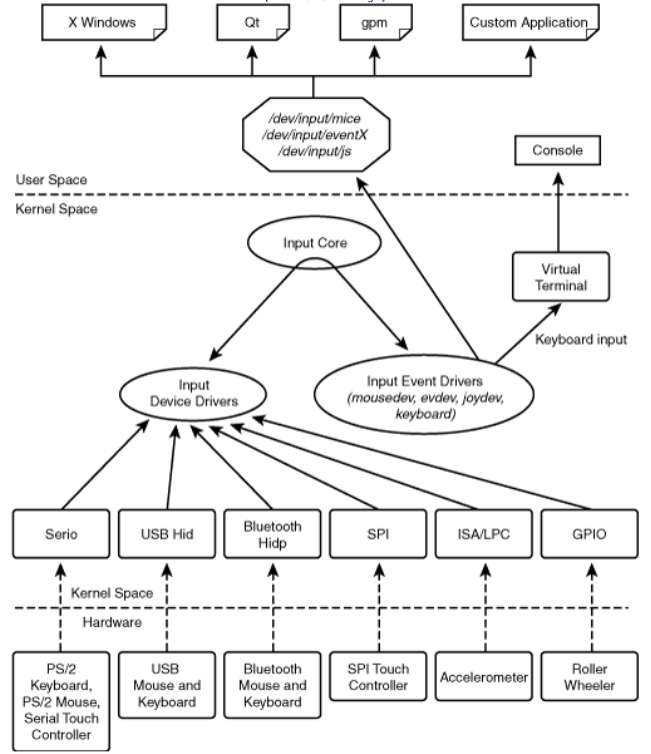
\includegraphics[width=0.7\linewidth]{src/img/input_system}
	\caption{Структура подсистемы ввода}
	\label{fig:inputsystem}
\end{figure}

\subsubsection{Драйверы событий для мыши}
Драйверы событий предлагают аппаратно независимую абстракцию для взаимодействия с устройствами ввода.
evdev (устройство события) - это общий интерфейс ввода событий в ядре Linux. 
Он обобщает необработанные события от драйверов устройств и делает их доступными через символьные устройства в каталоге /dev/input/. 

Каждое событие имеет структуру показаную в листинге \ref{lst:evdev}.

\begin{lstlisting}[caption=Структура события evdev, label=lst:evdev]
struct input_event {
	struct timeval time; 	// Timestamp
	\_\_u16 type; 			// Event type
	\_\_u16 code;				// Event code
	\_\_s32 value;			// Event value
}
\end{lstlisting}

Основные типы событий испускаемые evdev:
\begin{enumerate}
	\item EV\_SYN - разделение событий;
	\item EV\_KEY - для отображения нажатия клавиш клавиатуры, мыши или других кнопочных устройств;
	\item EV\_REL - передача относительного изменения координат, например при движении компьютерной мышью.
\end{enumerate}




